%\documentclass[class=article, float=false, crop=false]{standalone}
%\usepackage{standalone}
%\usepackage{varioref}

%\documentclass[10pt,letterpaper]{article}
%
%\input{error_control_of_enhanced_sampling-header}
%\begin{document}

\newlength{\heightMinusFoot}
\setlength{\heightMinusFoot}{\textheight-2cm}

\secnolabel{Figures}

%\tracingmacros=1
\begin{figure}[h]
    \begin{center}
    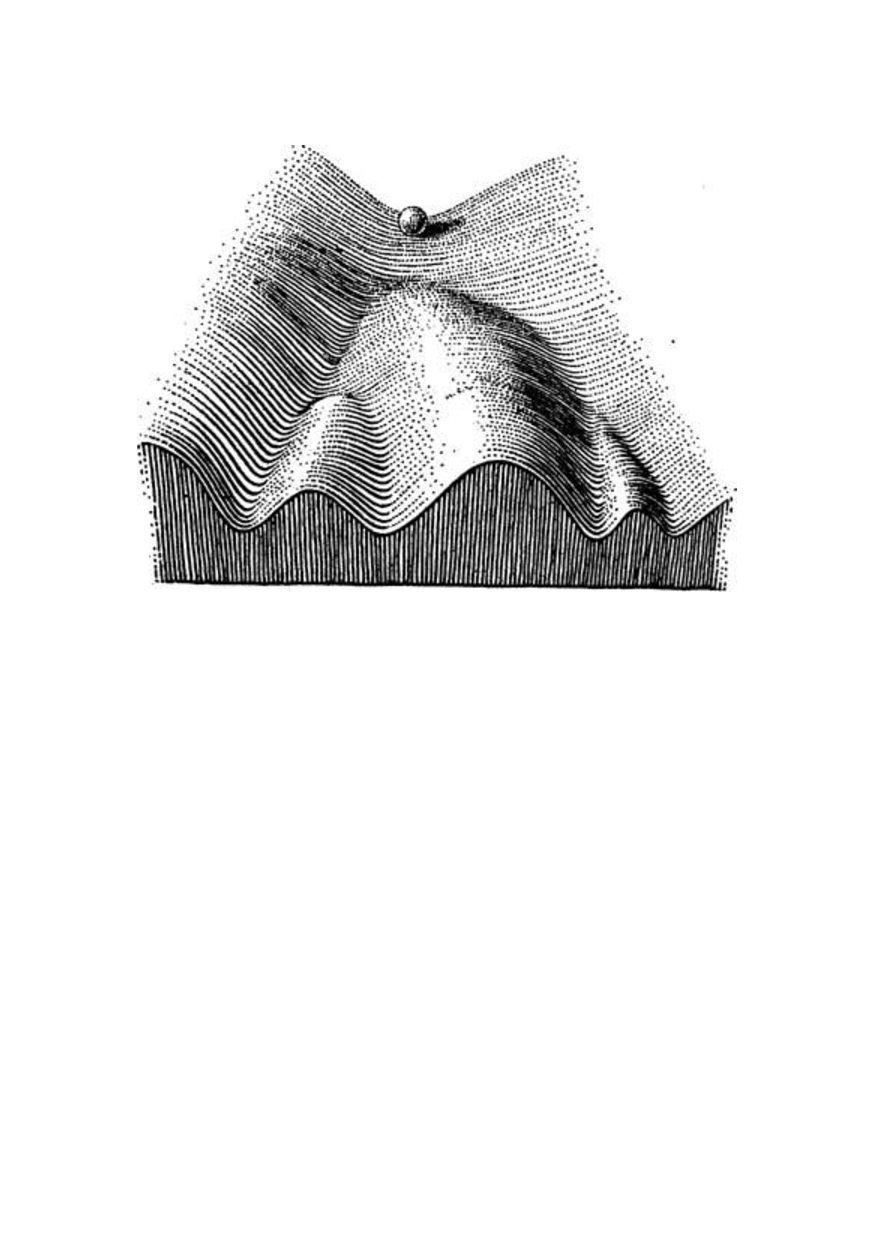
\includegraphics[width=8.45cm, height=\textheight, keepaspectratio]{{thesis_intro/figures/waddington_1957_chap2_fig4}.pdf}
    \end{center}
%    \tracingmacros=1
    \caption[The epigenetic landscape of a developing cell]{The epigenetic landscape of a developing cell, as envisioned by Waddington. The ball represents a cell at the beginning of development. Eventually the ball/cell will reach the bottom of the hill, ending up in one of several possible terminal cell types. The steep terrain counteracts most perturbations by forcing the ball back onto the path, making the whole process robust. Reprinted from Waddington, 1957\supercite{Waddington:1957ub}.}
%    \tracingmacros=0
    \label{fig:waddington_landscape}
\end{figure}
\clearpage

\begin{figure}[h]
    \begin{center}
    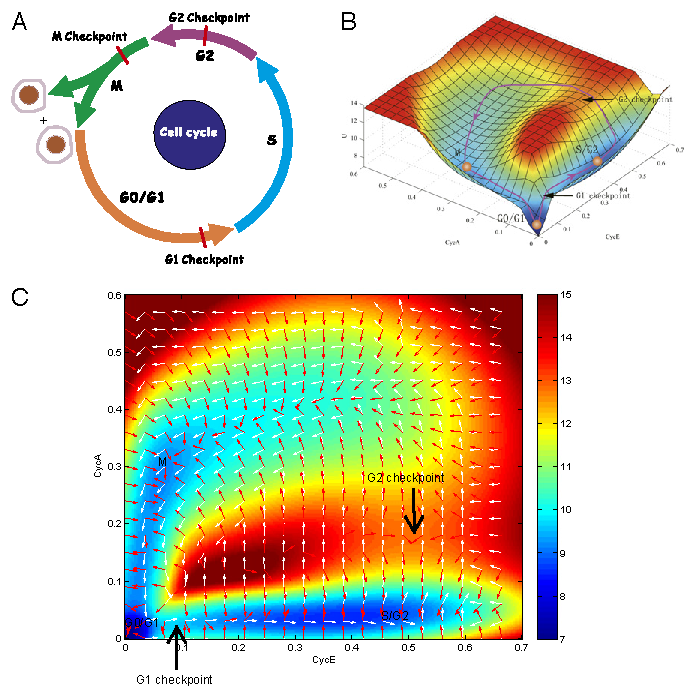
\includegraphics[width=8.45cm, height=\textheight, keepaspectratio]{{thesis_intro/figures/wang_2014_fig2}.pdf}
    \end{center}
    \caption[Three views of the mammalian cell cycle]{Three views of the mammalian cell cycle. A) The classical schematic view. B) The potential surface of the cell cycle. Data was taken from a 44 dimensional model and projected onto the concentrations of two cyclins, $CycA$ and $CycE$ (arbitrary units). The low points on the surface correspond to the various phenotypes along the cell cycle, and the transition path between them is shown. C) A 2D rendition of the complete epigenetic landscape of the model shown in B. The red arrows show the gradient of the potential, whereas the white arrows show the probability flux. Note that they never exactly coincide. Reprinted from Li et al., 2014\supercite{Li:2014iw}.}
    \label{fig:wang_cell_cycle_landscape}
\end{figure}
\clearpage

\begin{figure}[h]
    \begin{center}
    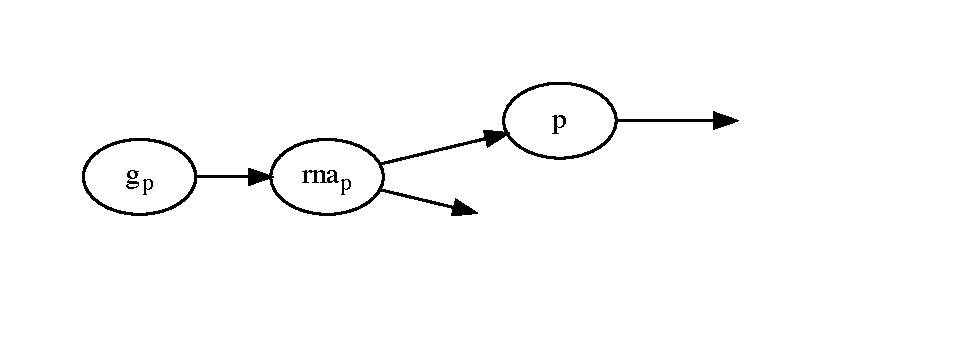
\includegraphics[keepaspectratio]{{thesis_intro/figures/simple_expression_digraph}.pdf}
    \end{center}
    \caption[A simple digraph representation of the simple gene expression model]{A simple digraph representation of the simple gene expression model from \eqref{eq:simple_expression}. An arrow from one species to another implies that the first species is involved in the production of the second. Arrows to empty space imply a decay reaction.}
    \label{fig:simple_expression_digraph}
\end{figure}
\clearpage

\begin{figure}[h]
    \begin{center}
    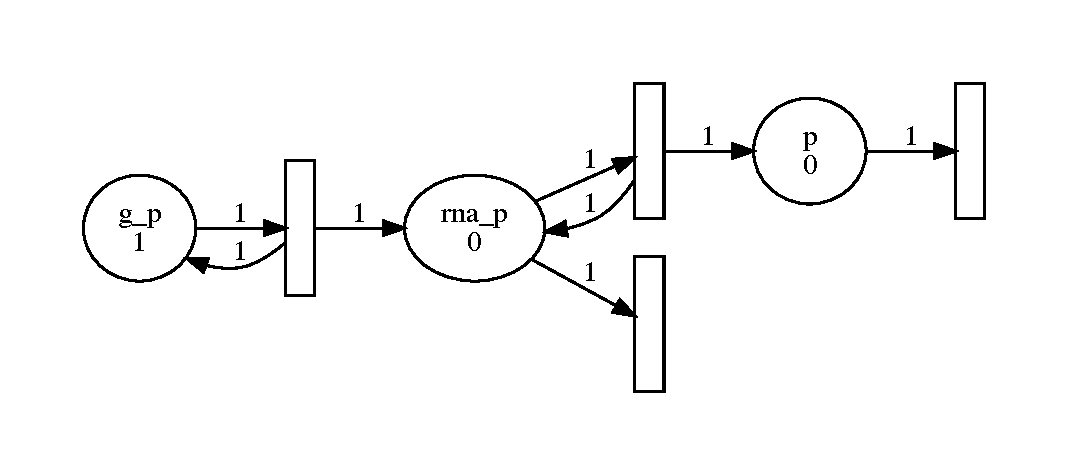
\includegraphics[width=1\textwidth,center]{{thesis_intro/figures/simple_expression_petri_net}.pdf}
    \end{center}
    \caption[A petri net representation of the simple genetic expression model]{A petri net representation of the simple genetic expression model from \eqref{eq:simple_expression}. Arrows starting at places (round nodes) and ending at transitions (rectangular nodes) imply that the connected species is a reactant in the connected reaction. Arrows starting at transitions and ending at places imply that the connected reaction produces the connected species. Above each arrow is a weight that gives its stoichiometry. The marking (the count of each species) is shown underneath the name of each species. Transitions that have no arrows leaving them imply a decay reaction.}
    \label{fig:simple_expression_petri_net}
\end{figure}
\clearpage

\begin{figure}[h]
    \begin{center}
    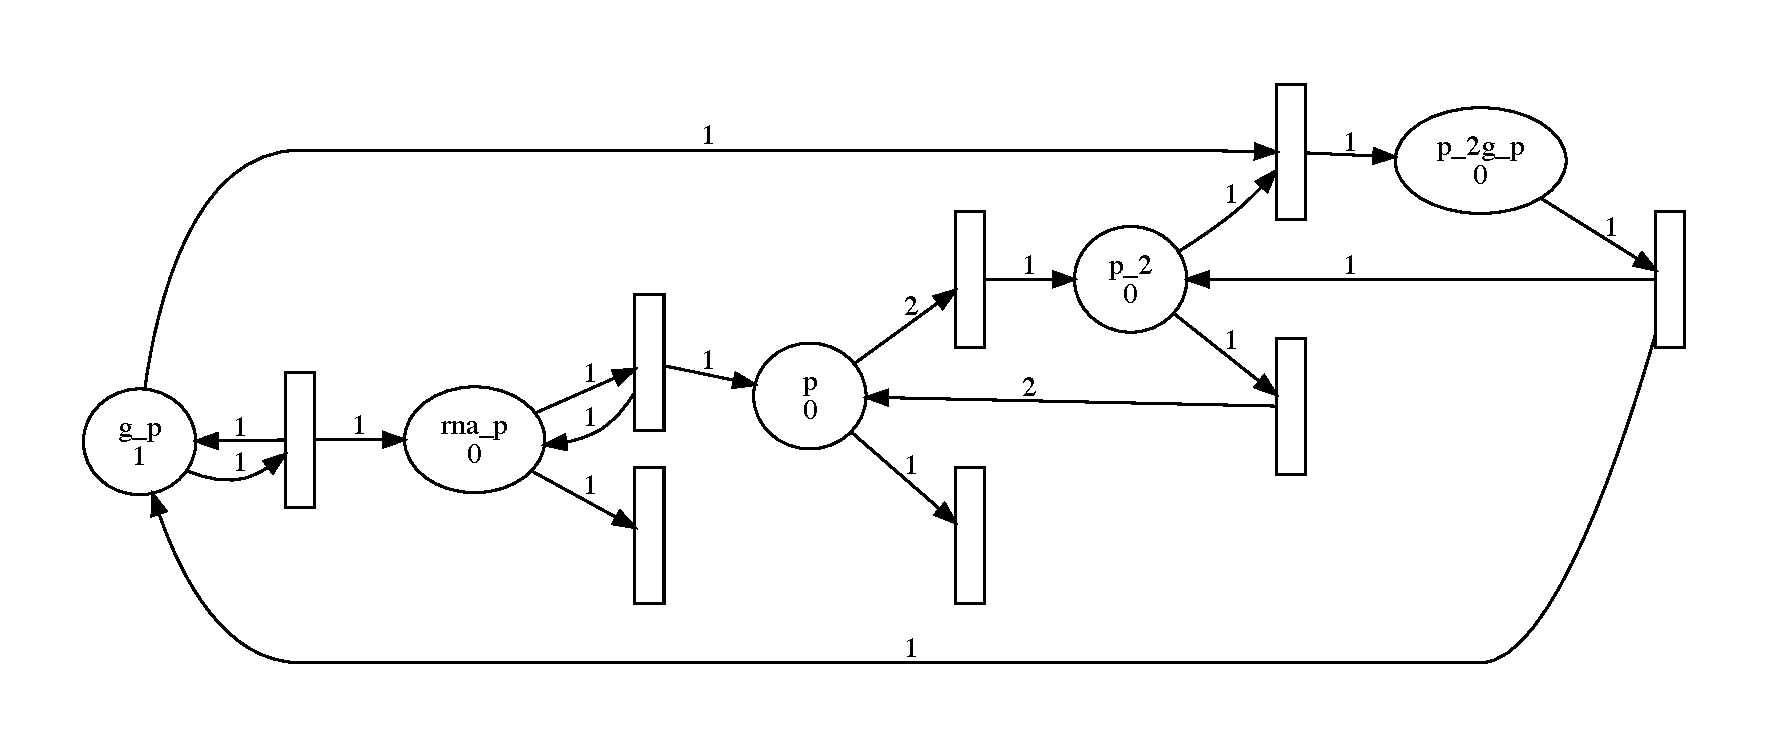
\includegraphics[width=1.2\textwidth,center]{{thesis_intro/figures/self_regulating_expression_petri_net}.pdf}
    \end{center}
    \caption[A petri net representation of the self regulating genetic expression model]{A petri net representation of the self regulating genetic expression model from \eqref{eq:self_regulating_expression}. The network is represented as described in \figref{fig:simple_expression_petri_net}.}
    \label{fig:self_regulating_expression_petri_net}
\end{figure}
\clearpage

\begin{figure}[h]
    \begin{center}
    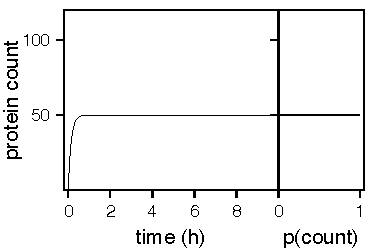
\includegraphics[keepaspectratio]{{thesis_intro/figures/simple_expression_timeseries_deterministic}.pdf}
    \end{center}
    \caption[Time series from a deterministic simulation of the simple expression system]{Time series from a deterministic simulation of the simple expression system (see \eqref{eq:simple_expression}) with ${ \condetx{1}=.1, \condetx{2}=.1, \condetx{3}=.1, \condetx{4}=2 \cdot 10^{-3} }$. The subplot along the left side shows the epigenetic landscape (as calculated via a histogram of the adjacent time series).}
    \label{fig:simple_expression_timeseries_deterministic}
\end{figure}
\clearpage

\begin{figure}[h]
    \begin{center}
    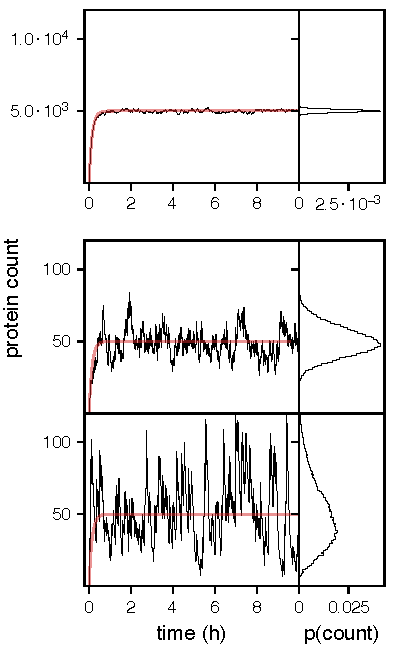
\includegraphics[keepaspectratio]{{thesis_intro/figures/simple_expression_timeseries_stochastic}.pdf}
    \end{center}
    \caption[Time series from stochastic simulations of the simple expression system]{(Black lines) time series from stochastic simulations of the simple expression system (see \eqref{eq:simple_expression}). The subplots along the left side show the epigenetic landscape of each variant (as calculated via a histogram of data from 10 simulation days, including the adjacent stochastic time series). (Red lines) the deterministic simulation of the same system, for comparison purposes. (Top panel) simple expression system with ${ \condetx{1}=10, \condetx{2}=.1, \condetx{3}=.1, \condetx{4}=2 \cdot 10^{-3} }$ (Middle panel) same, with ${ \condetx{1}=.1, \condetx{2}=.1, \condetx{3}=.1, \condetx{4}=2 \cdot 10^{-3} }$. (Bottom panel) same, with ${ \condetx{1}=.01, \condetx{2}=1, \condetx{3}=.1, \condetx{4}=2 \cdot 10^{-3} }$. The same constants were used in the deterministic and stochastic simulations (\ie $\constoch = \condet$). The mean expression level of the system simulated in the top panel is 100x that of the systems in the bottom two panels. From top to bottom the noise strengths are 1.98, 1.98, and 10.8039 (see \eqref{eq:simple_expression_noise_strength}).}
    \label{fig:simple_expression_timeseries_stochastic}
\end{figure}
\clearpage

\begin{figure}[h]
    \begin{center}
    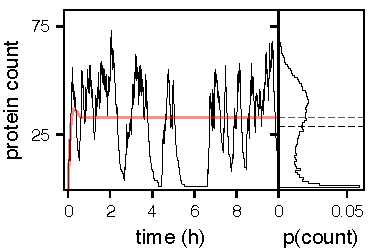
\includegraphics[keepaspectratio]{{thesis_intro/figures/self_regulating_expression_timeseries_stochastic}.pdf}
    \end{center}
    \caption[Time series from a stochastic simulation of the self regulating expression system]{(Black line) time series from a stochastic simulation of the self regulating expression system (see \eqref{eq:self_regulating_expression}). (Red line) the deterministic simulation of the same system. The subplot along the left side shows the epigenetic landscape. (Black and red dashed lines)  the mean protein expression value as calculated by stochastic and deterministic simulation, at $28.7$ and $33.0$ respectively ($15\%$ divergence). The deterministic rate constants used were ${ \condetx{1}=.1, \condetx{2}=.1, \condetx{3}=.1, \condetx{4}=2 \cdot 10^{-3}, \condetx{5}=10^{-6}, \condetx{6}=1, \condetx{7}=1, \condetx{8}=2 \cdot 10^{-3} }$. The stochastic rate constants were the same (\ie $\constoch = \condet$), except for $\constochx{5} = 2 \cdot \condetx{5} = 2 \cdot 10^{-6}$ (as per \eqref{eq:deterministic_second_order_self}).}
    \label{fig:self_regulating_expression_timeseries_stochastic}
\end{figure}
\clearpage

%\begin{figure}[h]
%    \begin{center}
%    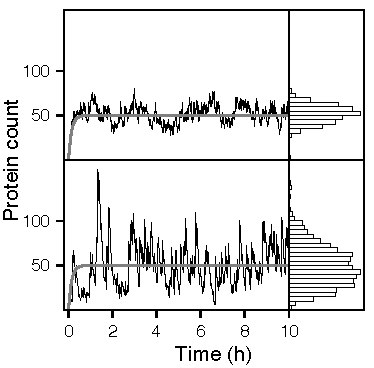
\includegraphics[keepaspectratio]{{thesis_intro/figures/simple_expression_timeseries_fixed_mean}.pdf}
%    \end{center}
%    \caption{(Black lines) time series from stochastic simulations of the simple expression system (see \eqref{eq:simple_expression}). The subplots along the left side show the epigenetic landscape of each variant (as calculated via a histogram of the stochastic time series). (Gray lines) the determistic simulation of the same system, for comparison purposes. (Top panel) simple expression system with ${ \condetx{1}=.1, \condetx{2}=.1, \condetx{3}=.1, \condetx{4}=.002 }$. (Bottom panel) same with ${ \condetx{1}=.01, \condetx{2}=1, \condetx{3}=.1, \condetx{4}=.002 }$. To first order, the noise scales\supercite{Ozbudak:2002iq} as $1 + \frac{\condetx{2}}{\condetx{3} + \condetx{4}}$.}
%    \label{fig:simple_expression_timeseries_fixed_mean}
%\end{figure}
%\clearpage

\begin{figure}[h]
    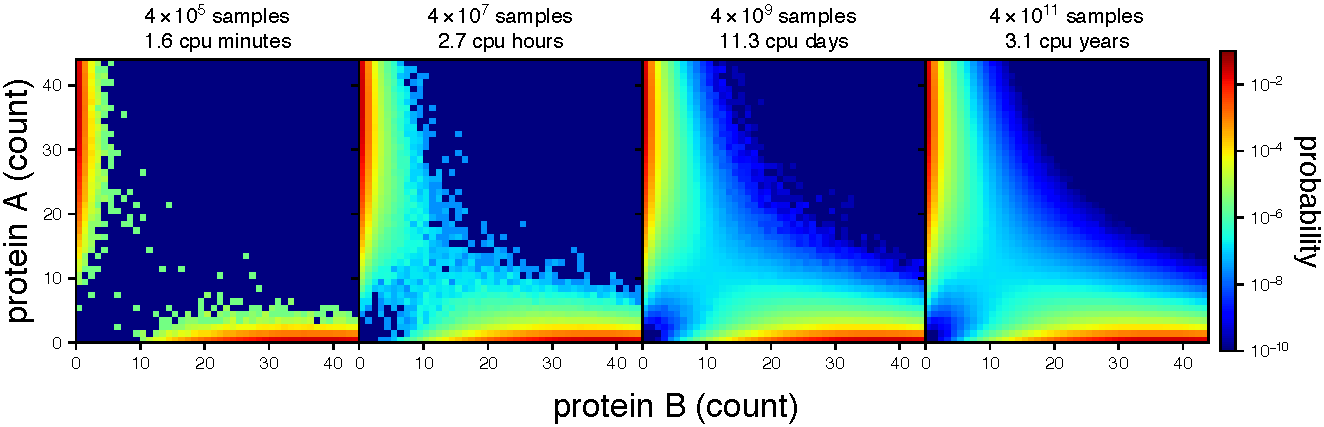
\includegraphics[width=1.2\textwidth,center]{{thesis_intro/figures/gts_theta_1en1_landscape_2d_comparison_samples}.pdf}
    \caption[Two dimensional epigenetic landscapes generated from the $\GTSSLOWEST$ system]{Two dimensional epigenetic landscapes generated from the $\GTSSLOWEST$ system (described in \secref{sec:gts}\todo{format in ECES paper so the preceeding secref works}). From left to right, the subplots show versions of the same landscape calculated using an increasing number of species count samples. The total sample count used in each landscape, and the CPU time used to collect those samples, is shown above each subplot. The samples were taken from 20 trajectories, each of which was generated using several thousand CPU cores running a parallelized implementation of \abr{SSA}\supercite{Roberts:2013cu}.}
    \label{fig:gts_theta_1en1_landscape_2d_comparison_samples}
\end{figure}
\clearpage

%\begin{figure}[h]
%    \begin{center}
%    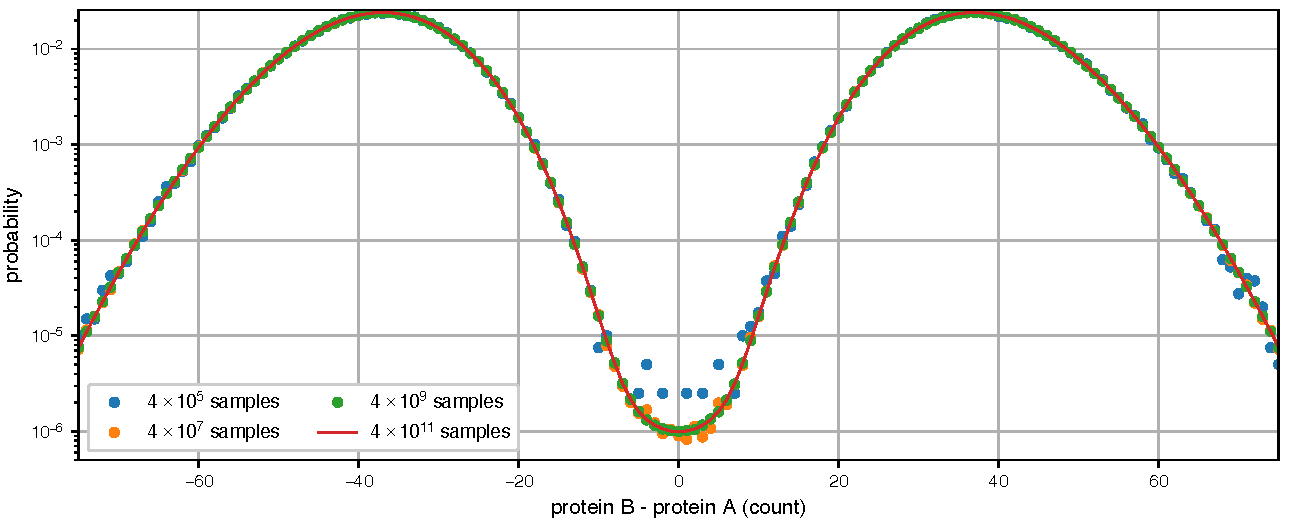
\includegraphics[width=1.2\textwidth,center]{{thesis_intro/figures/gts_theta_1en1_landscape_1d_comparison_samples}.pdf}
%    \end{center}
%    \caption{One dimensional versions of the two dimensional landscapes shown in \figref{fig:gts_theta_1en1_landscape_2d_comparison_samples}, shown overlapping for ease of comparison. The largest divergence between the landscapes calculated with different sample counts can be seen in the middle of the transition region, at $x=0$.}
%    \label{fig:gts_theta_1en1_landscape_1d_comparison_samples}
%\end{figure}
%\clearpage

\begin{figure}[h]
    \begin{center}
    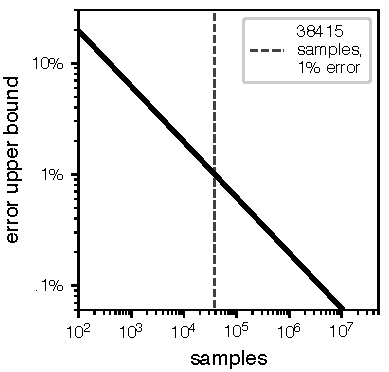
\includegraphics[keepaspectratio]{{thesis_intro/figures/sampling_error_mean_of_exponential}.pdf}
    \end{center}
    \caption[The margin of error vs sample count when using stochastic simulation to calculate the \abr{MFPT} of a rare state switching event]{The margin of error ($95\%$ confidence) vs sample count when using stochastic simulation to calculate the \abr{MFPT} of a rare state switching event. The x-axis begins at $100$ in order to emphasize that the relationship is only valid in the limit of large sample size. See \secref{sec:moe_from_simulation_params}\todo{make the preceding secref from intro to paper work} for derivation and details.}
    \label{fig:sampling_error_mean_of_exponential}
\end{figure}
\clearpage

\begin{figure}[h]
    \begin{center}
    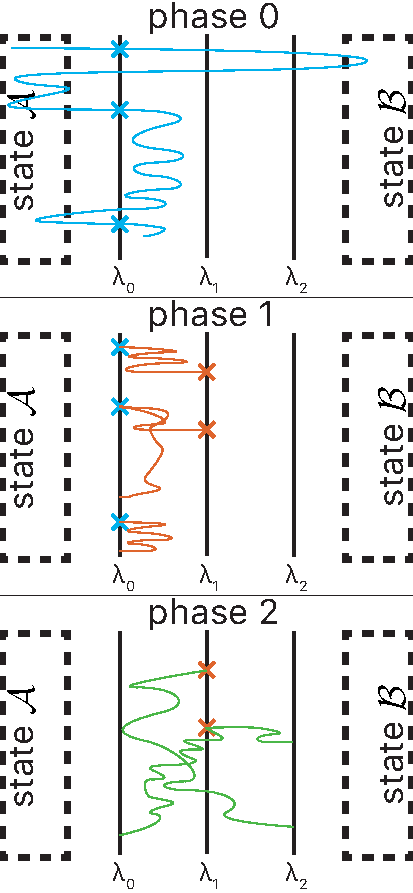
\includegraphics[keepaspectratio]{{thesis_intro/figures/fflux_stages}.pdf}
    \end{center}
    \caption[A schematic representation of an \abr{FFS} simulation run from $\atob$]{A schematic representation of an \abr{FFS} simulation run from $\atob$. The simulation shown has 3 phases, one for each interface $\ifacei$ that is defined.\todo{maybe?: explain that simulation time increases towards the bottom of the y-axis on each subplot} During each phase $\phasegz$, trajectories are initialized from one of the points (chosen at random) where a trajectory in the previous phase crossed $\ifaceimo$ while traveling in the forward direction (\ie towards $\stateb$). During phase $2$ (the final phase), trajectories that cross $\ifacex{2}$ are considered to have completed the transition into $\stateb$.}
    \label{fig:fflux_stages}
\end{figure}
\clearpage

\begin{figure}[h]
    \begin{center}
    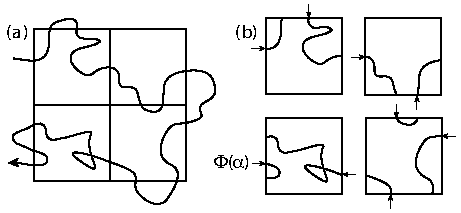
\includegraphics[keepaspectratio]{{thesis_intro/figures/dickson_2009_fig2}.pdf}
    \end{center}
    \caption{Reprinted from Dickson et al., 2004\supercite{Dickson:2009gt}.}
    \label{fig:dickson_2009_fig2}
\end{figure}
\clearpage

\begin{figure}[h]
    \begin{center}
    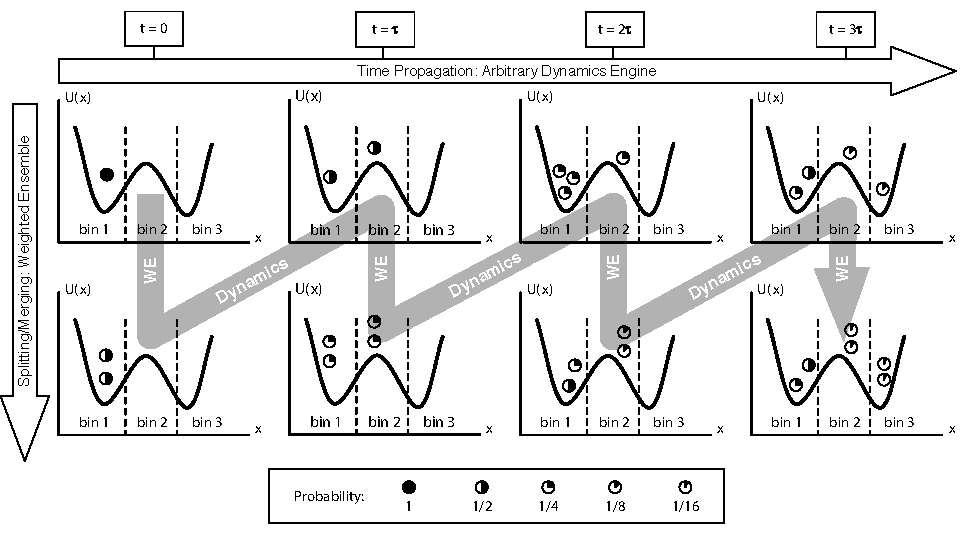
\includegraphics[width=1\textwidth,center]{{thesis_intro/figures/donovan_2013_fig1}.pdf}
    \end{center}
    \caption{Reprinted from Donovan et al., 2013\supercite{Donovan:2013gz}.}
    \label{fig:donovan_2013_fig1}
\end{figure}
\clearpage